\documentclass[]{article}
\newcommand{\FileDepth}{../../..}
\usepackage[letterpaper, landscape, margin=0.5cm]{geometry}
\usepackage[T1]{fontenc}
\usepackage{textcomp}%Not strictly necessary, but gives \textmu command for "micro."
\usepackage{fancyhdr}
\usepackage{amsmath}
\usepackage{amssymb}
\usepackage{graphicx}
\usepackage{xcolor}
\usepackage{tikz}
\usetikzlibrary{calc}
\usepackage[shortlabels]{enumitem}
\usepackage{multicol}
\usepackage{vwcol}
\usepackage{hyperref}
\usepackage{wrapfig}
%opening
\newcommand{\SecType}{L}
\newcommand{\Week}{11}
\title{PH 211 Lecture \Week}
\author{Benjamin Bauml}
\date{Summer 2024}

\newcommand{\Purpose}{4}
\newcommand{\DefOnly}{0}

\input{\FileDepth/Formats/Assignment20240614.tex}
\usepackage[absolute]{textpos}
% This package relies on Assignment Format 2024-06-14 or later to work. It is recommended that the Purpose and DefOnly commands be given as such:
%\newcommand{\Purpose}{4}
%\newcommand{\DefOnly}{0}
% Activities need to be entered outside of the TeacherMargin and PresentSpace environments, otherwise they will be defined only locally. They can even go in the preamble.
\newenvironment{TeacherMargin}{\begin{textblock*}{10.8cm}(0.5cm,0.5cm)
\small}{\end{textblock*}
\hspace{0.1cm}}
\newenvironment{PresentSpace}{\begin{textblock*}{0.3cm}(26.85cm,9.35cm)
--
\end{textblock*}
\begin{textblock*}{15.6cm}(11.8cm,0.5cm)
\begin{Repurpose}{1}
\Large}{\end{Repurpose}
\end{textblock*}
\hspace{0.1cm}}

%\newcommand{\FBDaxes}[4][2]{
	\begin{scope}[shift={(#2)},rotate=#3]
		% x-axis
		\draw[thick,->] (-#1,0) -- (#1,0);
		\node[anchor=west] at (#1,0) {$x$};
		% y-axis
		\draw[thick,->] (0,-#1) -- (0,#1);
		\node[anchor=south] at (0,#1) {$y$};
		\coordinate (#4) at (0,0);
	\end{scope}
}
\newcommand{\FBDvectorMA}[4]{
	\begin{scope}[shift={(#1)}]
		\coordinate (#4tip) at ({#2*cos(#3)},{#2*sin(#3)});
		\draw[ultra thick,blue,->] (#1) -- (#4tip);
	\end{scope}
}
\newcommand{\FBDvectorXY}[3]{
	\begin{scope}[shift={(#1)}]
		\coordinate (#3tip) at (#2);
		\draw[ultra thick,blue,->] (0,0) -- (#3tip);
	\end{scope}
}
\newcommand{\FBDdot}[1]{
	\filldraw[black] (#1) circle (3pt);
}
\newcommand{\FBDbox}[5][1]{
	\begin{scope}[shift={(#2)},rotate=#3]
		\filldraw[color=black,fill=white,thick] ({-#1/2},{#1/2}) -- ({-#1/2},{-#1/2}) -- ({#1/2},{-#1/2}) -- ({#1/2},{#1/2}) -- cycle;
		% Left side coordinates
		\coordinate (#4ltq) at ({-#1/2},{#1/4});
		\coordinate (#4lcent) at ({-#1/2},0);
		\coordinate (#4lbq) at ({-#1/2},{-#1/4});
		% right side coordinates
		\coordinate (#4rtq) at ({#1/2},{#1/4});
		\coordinate (#4rcent) at ({#1/2},0);
		\coordinate (#4rbq) at ({#1/2},{-#1/4});
		% top coordinates
		\coordinate (#4tlq) at ({-#1/4},{#1/2});
		\coordinate (#4tcent) at (0,{#1/2});
		\coordinate (#4trq) at ({#1/4},{#1/2});
		% bottom coordinates
		\coordinate (#4blq) at ({-#1/4},{-#1/2});
		\coordinate (#4bcent) at (0,{-#1/2});
		\coordinate (#4brq) at ({#1/4},{-#1/2});
		% corners
		\coordinate (#4tl) at ({-#1/2},{#1/2});
		\coordinate (#4tr) at ({#1/2},{#1/2});
		\coordinate (#4bl) at ({-#1/2},{-#1/2});
		\coordinate (#4br) at ({#1/2},{-#1/2});
		\node at (0,0) {#5};
	\end{scope}
}
%\newcommand{\MVec}[3][0]{%Creates a momentum vector of length #3 centered at #2 and rotated #1 degrees counterclockwise.
	\begin{scope}[rotate=#1,shift={(#2)}]
		\draw[->,thick] ({-#3/2},0) -- ({#3/2},0);
	\end{scope}
}
\newcommand{\MDot}[1]{%Creates a dot at #1 to represent a zero vector.
	\filldraw (#1) circle (1pt);
}
\newcommand{\MVDRows}[2][4.5]{%Creates the rows (initial, delta, final) of a momentum vector diagram. The optional argument determines the width of the table, and defaults to a good length for three columns (two objects and the total system). The non-optional argument gives a coordinate name (not displayed) to the diagram.
	\begin{scope}
		%\draw[thick] (0,5.5) -- (0,0);
		\draw[thick] (-1,4.5) -- (#1,4.5);
		\node at (-0.5,3.75) {$\vec{p}_{i}$};
		\draw[thick] (-1,3) -- (#1,3);
		\node at (-0.5,2.25) {$\Delta\vec{p}$};
		\draw[thick] (-1,1.5) -- (#1,1.5);
		\node at (-0.5,0.75) {$\vec{p}_{f}$};
		\coordinate (#2) at (0,5);
	\end{scope}
}
\newcommand{\MVDCol}[4][0.75]{%Creates a column for an object in a momentum vector diagram. The first (non-optional) argument is the coordinate name (not displayed) of the column, while the second is the displayed column header. The first argument also names the three entries down the column. The third argument anchors the column, so it should either be the coordinate name of the MVD (for the first column) or the coordinate name of the previous column. The optional argument indicates how far the center of the column should be from the previous column's edge, and defaults to 0.75.
	\begin{scope}[shift={(#4)}]
		\node at (#1,0) {#3};
		%\draw[thick] ({#1*2},0.5) -- ({#1*2},-5);
		\draw[thick] (0,0.5) -- (0,-5);
		\coordinate (#2init) at (#1,-1.25);
		\coordinate (#2delt) at (#1,-2.75);
		\coordinate (#2fin) at (#1,-4.25);
		\coordinate (#2) at ({#1*2},0);
	\end{scope}
}

%\input{\FileDepth/Activities/Activity_One/Activity_One.tex}
%\input{\FileDepth/Activities/Activity_Two/Activity_Two.tex}

\begin{document}
\begin{TeacherMargin}

\end{TeacherMargin}
\begin{PresentSpace}
\begin{center}
	\huge Lecture \Week: Laws of Motion
\end{center}
\vspace{0.5cm}
\underline{Warm-Up Activity} \\
Question?
%\begin{multicols}{2}
\begin{enumerate}[(A)]
	\item Answer?
\end{enumerate}
%\end{multicols}
\end{PresentSpace}
\newpage
\begin{TeacherMargin}
\begin{center}
	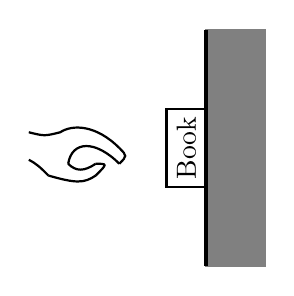
\begin{tikzpicture}
		\filldraw[gray] (0,-1.5) rectangle (0.75,1.5);
		\draw[ultra thick] (0,1.5) -- (0,-1.5);
		\draw[thick] (-0.5,-0.5) rectangle (0,0.5);
		\node[rotate=90] at (-0.25,0) {Book};
		\begin{scope}[shift={(-2,0)}]
			\draw[thick] (-0.25,0.2) .. controls (-0.05,0.15) .. (0.15,0.2) .. controls (0.3,0.3) and (0.6,0.3) .. (0.9,0);
			\draw[thick] (0.9,0) .. controls (1,-0.1) .. (0.9,-0.2);
			\draw[thick,shift={(0,-0.2)}] (0.25,0) .. controls (0.3,0.3) and (0.6,0.3) .. (0.9,0);
			\draw[thick] (0.25,-0.2) .. controls (0.35,-0.3) and (0.45,-0.3) .. (0.6,-0.2);
			\draw[thick] (0.6,-0.2) .. controls (0.75,-0.2) .. (0.6,-0.35);
			\draw[thick,shift={(0,-0.15)}] (0,-0.2) .. controls (0.35,-0.3) and (0.45,-0.3) .. (0.6,-0.2);
			\draw[thick,shift={(0,-0.35)}] (-0.25,0.2) .. controls (-0.15,0.15) and (-0.1,0.1) .. (0,0);
		\end{scope}
	\end{tikzpicture}
\end{center}
\end{TeacherMargin}
\begin{PresentSpace}
\vspace{-10pt}
\section*{L\Week-1: Book on the Wall -- Hold Still}
\vspace{-10pt}
\begin{itemize}
	\item You push a book against a vertical wall so the book does not move.
	\begin{itemize}
		\item Sketch a picture of the book and the wall.
		\item Identify and describe each force acting on the book.
		\item Draw and label a free-body diagram for the book.
	\end{itemize}
	\item What do you know about the magnitudes of the forces acting on the book?
	\item What happens to each force if you push harder?
\end{itemize}
\end{PresentSpace}
\newpage
\begin{TeacherMargin}

\end{TeacherMargin}
\begin{PresentSpace}
\vspace{-10pt}
\section*{L\Week-2: Book on the Wall -- Slide Down}
\vspace{-10pt}
\begin{itemize}
	\item You push a different book horizontally against a vertical wall so that the book slides downward at constant speed.
	\item You know the coefficients of friction are $\mu_{bw}$ (between the book and the wall) and \textit{zero} (between the book and your hand). You also know the mass $m$ of the book.
	\begin{itemize}
		\item Draw a free-body diagram for this situation.
		\item Determine the magnitude of the force that your hand must exert on the book.
		\item Make sense of your answer in at least three different ways.
	\end{itemize}
\end{itemize}
\end{PresentSpace}
\newpage
\begin{TeacherMargin}
	
\end{TeacherMargin}
\begin{PresentSpace}
\section*{Main Ideas}
\begin{itemize}
	\item There are many different \textit{kinds} of forces that we can analyze differently.
	\item Objects can only change their motion when acted upon by an external force.
	\item The net force on an object is equal to its mass times its acceleration.
	\item Forces are vectors.
	\item When more than one force acts on an object, we can add all the forces together.
	\item We can model forces quantitatively.
	\item When an object is at rest or moving at constant speed, the forces balance and the object is in equilibrium.
\end{itemize}
\end{PresentSpace}
\end{document}